\section{Estado del arte}

En esta sección, el objetivo es analizar la literatura reciente y los artículos publicados sobre el entrenamiento de modelos de aprendizaje profundo, tanto a través de técnicas basadas en gradiente descendente como metaheurísticas, enfocándonos en las familias de modelos ConvNets y MLP. Para un mejor contexto, realizaremos una búsqueda en la base de datos de referencias bibliográficas y citas SCOPUS, con el fin de conocer el estado actual de la literatura. La primera búsqueda será simple y general para obtener una visión global sobre el entrenamiento de modelos de aprendizaje profundo.


\begin{verbatim}

TITLE-ABS-KEY ( deep  AND learning  AND training )
AND ( LIMIT-TO ( SUBJAREA ,  "COMP" ) ) 

\end{verbatim}


El total de artículos para esta búsqueda asciende a 78,378 resultados, cuya tendencia puede apreciarse en la figura \ref{fig:scopus_deep}. En ella se observa un punto de inflexión en el año 2012, cuando las publicaciones anuales comienzan a crecer de manera exponencial, siendo prácticamente nulas previamente. Este año es significativo porque AlexNet ganó la competición de \textit{ImageNet}\footnote{\url{https://www.image-net.org/challenges/LSVRC/}}, marcando un aumento muy significativo del interés por las redes neuronales profundas a partir de entonces.

\begin{figure}
    \centering
    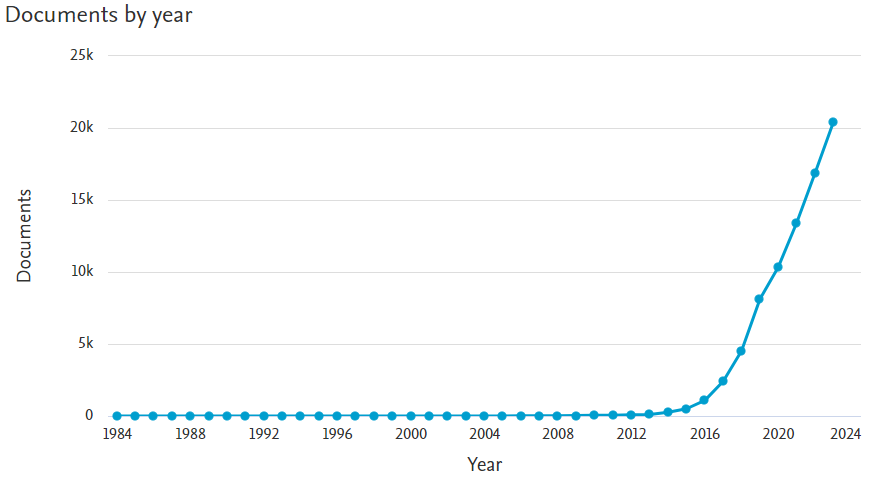
\includegraphics[width=0.75\linewidth]{Plantilla_TFG_latex//imagenes//Inf//EdA/scopus_deep.png}
    \caption{Números de artículos publicados por año en la web SCOPUS para la búsqueda TITLE-ABS-KEY ( deep  AND learning  AND training ), muestra el número de artículos por año.}
    \label{fig:scopus_deep}
\end{figure}

Ahora vamos a realizar una búsqueda en el ámbito del entrenamiento de modelos de aprendizaje profundo, diferenciando entre técnicas clásicas y técnicas metaheurísticas. Para ello, utilizaremos términos definitorios y los nombres de las técnicas empleadas en este TFG, realizando las siguientes búsquedas:

\begin{verbatim}
	TITLE-ABS-KEY ( ( deep  AND  learning )  AND  training  AND 
	( metaheuristic  OR  metaheuristics  OR  shade  OR  shade-ils 
	OR  ( differential  AND  evolution )  OR  memetic  OR 
	genetic ) )  AND  ( LIMIT-TO ( SUBJAREA ,  "COMP" ) )

\end{verbatim}

\begin{verbatim}
	TITLE-ABS-KEY ( ( deep  AND  learning )  AND  training  AND 
	( gradient  OR  adam  OR  optimizer  OR  rmsprop  OR  nag ) )  
	AND  ( LIMIT-TO ( SUBJAREA ,  "COMP" ) ) 
\end{verbatim}

\begin{figure}[!tbp]
  \centering
  \subfloat{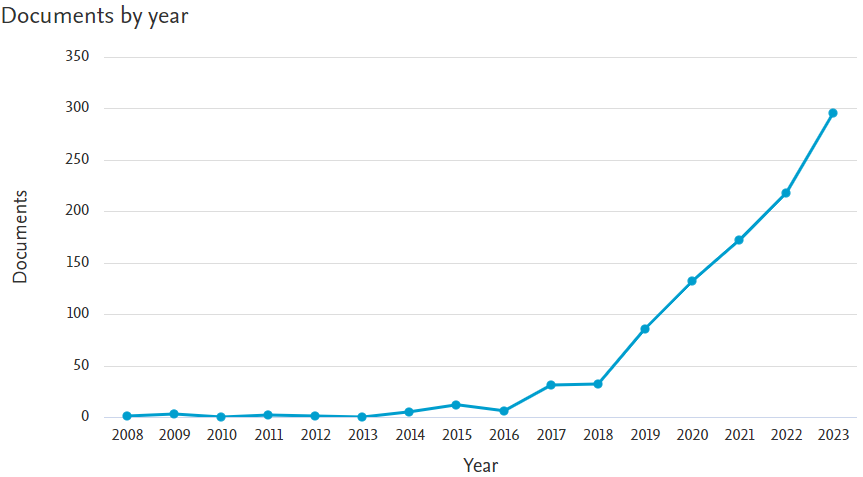
\includegraphics[width=0.75\textwidth]{Plantilla_TFG_latex//imagenes//Inf//EdA/scopus_mh.png}}
  \hfill
  \subfloat{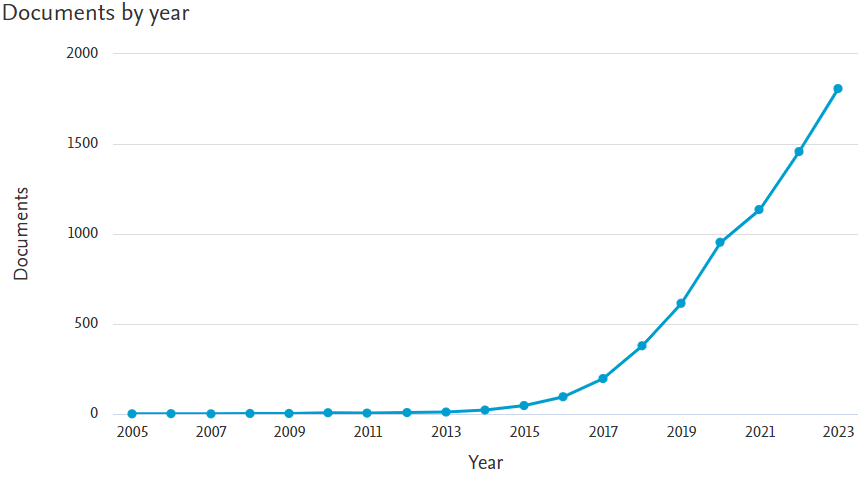
\includegraphics[width=0.75\textwidth]{Plantilla_TFG_latex//imagenes//Inf//EdA/scopus_gd.png}}
  \caption{Número de arrtículos publicados por año para el entrenamiento de modelos de aprendizaje profundo con metaheurísticas (arriba) y gradiente descendente (debajo) según las búsquedas correspondientes.}
  \label{fig:resEdA}
\end{figure}

Obtenemos una cantidad de 6,753 artículos en lo referente al entrenamiento de modelos de aprendizaje profundo con técnicas basadas en gradiente descendente y 997 para técnicas metaheurísticas. Vemos que la diferencia entre ambas cantidades es considerable, siendo la primera 7 veces mayor que la segunda. Destacamos sin embargo que la tendencia en ambos casos es muy similar, como se observa en la figura \ref{fig:resEdA}, aumentando prácticamente en la misma proporción desde el año 2012.



\subsection{Gradiente descendente y optimizadores}

El gradiente descendente es el algoritmo de aprendizaje utilizado por defecto en prácticamente todas las tareas de aprendizaje profundo, gracias a su eficiencia y buenos resultados. Los problemas que surgen en su convergencia se intentan evitar en la práctica mediante el desarrollo de modificaciones a su algoritmo, denominadas optimizadores. La literatura en este ámbito es extensa, con una gran variedad de optimizadores disponibles. A continuación, realizaremos una distinción clara entre optimizadores de primer y de segundo orden.


Aunque los optimizadores de segundo orden presentan mejores propiedades teóricas y ofrecen una convergencia más rápida y estable al utilizar más información del problema, el cálculo o la aproximación de la matriz Hessiana incrementa significativamente el poder computacional necesario para su uso, lo que ralentiza el entrenamiento. Además, hay un problema de memoria: para una red neuronal con 1 millón de parámetros, se requeriría almacenar una matriz de tamaño $1,000,000 \times 1,000,000$, que ocuparía aproximadamente 3,725 GB de memoria RAM. Esto resulta inviable, especialmente considerando que en el top-10 de modelos de clasificación de la competición \textit{ImageNet}, ningún modelo tiene menos de mil millones de parámetros.

Incluso si eliminamos estos inconvenientes de memoria con métodos como L-BFGS (ver sección \ref{sec:l-bfgs}), enfrentamos un problema significativo: estos métodos requieren el cálculo del gradiente sobre todos los datos de entrenamiento. Conjuntos como \textit{ImageNet}, que contienen más de un millón de ejemplos, hacen que esto sea computacionalmente inviable. Conseguir que este tipo de algoritmos como L-BFGS funcionen con lotes es más complejo que en MBGD y de hecho es un área abierta de investigación.

En la práctica no es común ver el algoritmo L-BFGS u otros optimizadores de segundo orden aplicados a modelos de apendizaje profundo a gran escala. En su lugar se utilizan variantes de MBGD basadas en el uso de momento y en tasas de aprendizaje adaptativas, ya que son mucho más simples y más escalables. Existen varias opciones bastante asentadas, que forman parte de las librerías de aprendizaje automático más usadas como PyTorch y TensorFlow, entre las cuales destacan Adam, NAG, RMSProp, AdaGrad o SGD con momento. Vamos a analizar una comparativa\footnote{\url{https://akyrillidis.github.io/2020/03/05/algo.html}} entre los optimizadores de gradiente descendente con rendimiento del estado del arte para obtener una visión general.

En ella se diferencia entre los algoritmos que tienen tasa de aprendizaje adaptativa (Adam, AMSGrad, AdamW, QHAdam, Demon Adam, YellowFin) y los que no (SGDM, AggMo, QHM, Demon Momentum). Los modelos y conjuntos de datos usados en este análisis pueden observarse en la tabla \ref{table:exp}. Una consideración muy importante que se realiza en dicha comparativa, y que es bien sabida en el campo del aprendizaje automático, es que el rendimiento de una técnica de entrenamiento está muy ligado al dominio específico del problema. Puede ocurrir que un método que no sea de los mejores en términos generales sí lo sea en un problema específico. Pasamos ahora a describir rápidamente las técnicas más interesantes.

\begin{table}[]
\begin{tabular}{|c|c|}
\hline
\textbf{Dataset} & \textbf{Modelo}  \\ \hline
CIFAR-10          & ResNet18         \\ \hline
CIFAR-100         & VGG16            \\ \hline
STL10            & Wide ResNet 16-8 \\ \hline
F-MINST           & CAPS             \\ \hline
PTB              & LSTM             \\ \hline
MNIST            & VAE              \\ \hline
\end{tabular}
\caption{Tabla con los datasets utilizados con sus respectivos modelos en la experimentación de la comparativa (enlace)}
\label{table:exp}
\end{table}

YellowFin \cite{yellowfin} es un optimizador con tasa de aprendizaje y momento adaptativos, de manera que mantiene dichos hiperparámetros en un intervalo donde el ratio de convergencia es una constante igual a la raíz del momento. AdamW es una extensión de Adam en la que se utiliza penalización en los pesos del modelo de manera que exista un sesgo hacia valores más pequeños de los mismos durante el entrenamiento, ya que normalmente se asocian valores grandes en los parámetros con el sobreajuste. Aunque Adam ya incorpora este mecanismo, AdamW realiza una pequeña modificación a través de desacoplar esta penalización de la actualización del gradiente, resultando en un impacto notable. 

QHM es una extensión del método de momento clásico que introduce un término cuasi-hiperbólico. Esto permite una mezcla controlada entre el momento y el algoritmo de descenso de gradiente original, proporcionando una mayor flexibilidad y mejorando la estabilidad del entrenamiento. QHAdam combina las ventajas del optimizador Adam con las del descenso de gradiente con momento cuasi-hiperbólico. Introduce factores de amortiguación para controlar la contribución de las medias móviles de primer y segundo orden, ofreciendo un equilibrio entre estabilidad y rapidez en la convergencia. 

Demon Adam es una variante de Adam que ajusta dinámicamente el momento durante el entrenamiento. Utiliza una estrategia de decaimiento del momento para mejorar la adaptación a diferentes fases del entrenamiento, permitiendo una mejor convergencia y evitando caer en mínimos locales. Similar a Demon Adam, Demon Momentum aplica la técnica de decaimiento del momento, pero se usa con optimizadores basados solo en el momento clásico, no en Adam. Mejora la capacidad de adaptación del optimizador durante el entrenamiento al ajustar el momento de manera dinámica. AggMo  combina múltiples trayectorias de momento con diferentes factores de decaimiento. Esto ayuda a mejorar la exploración del espacio de parámetros y a mitigar la dependencia de los hiperparámetros del momento, proporcionando una convergencia más robusta y rápida.


Como conclusión, y atendiendo siempre al dominio específico del problema, se establece que YellowFin es la mejor opción en caso de no disponer de recursos para ajustar los hiperparámetros, ya que adapta el momento y la tasa de aprendizaje a lo largo del entrenamiento. Si se dispone de recursos, pero no demasiados, lo mejor son algoritmos de tasa de aprendizaje adaptativa de manera que sólo se tenga que ajustar el valor del momento; en concreto destacan AdamW, QHAdam y Demon Adam. En cambio si se quiere obtener el mejor rendimiento a toda costa, invirtiendo muchos recursos en el ajuste de parámteros, usar MBGD con momento es la mejor opción, aunque sea un método más clásico.


\subsection{Metaheurísticas en el entrenamiento de modelos}

Aún con el uso de optimizadores, hay ciertos inconvenientes en el entrenamiento que son insalvables, como los que están provocados por los cálculos del gradiente con el algoritmo de \textit{backpropagation}. Las técnicas metaheurísticas son una gran alternativa, ya que sus operadores de búsqueda no dependen de \textit{backpropagation}, evitando así sus problemas. 

Uno de los enfoques de aplicación de estas técnicas es la combinación con las técnicas clásicas, utilizando diferentes aproximaciones. Por ejemplo en \cite{162} se usa el algoritmo \textit{Artificial Bee Colony} \cite{beesalgo} sobre un conjunto de soluciones aleatorias para generar una población inicial de conjuntos de parámetros de un modelo que se entrenan con gradiente descendente. En \cite{155} se combina un algoritmo genético con el gradiente descendente, de manera que las nuevas soluciones son generadas con el operador de búsqueda del primero pero son evaluadas tras realizar varias épocas con el segundo. De manera similar en \cite{163} se usa la técnica metaheurística \textit{Particle Swarm Optimization} \cite{pso} para entrenar los parámetros de la última capa de una ConvNet, mientras que el resto se entrenan a través del algoritmo de gradiente descendente. La comparación arroja que la hibridación de ambas técnicas alcanza mejores resultados en términos de rapidez de convergencia y de \textit{accuracy}. Prácticamente la totalidad de la literatura referente a esta estrategia está centrada en ConvNets.

El otro enfoque es entrenar el modelo usando exclusivamente algoritmos bio-inspirados. En este ámbito destacan los estudios \cite{174} y \cite{176}, en los que se proponen dos técnicas basadas en \textit{Simulated Annealing} \cite{siman} para entrenar los parámetros de una ConvNet, consiguiendo mejor rendimiento y mayor velocidad de convergencia que en el mismo modelo entrenado mediante el algoritmo de gradiente descendente. Al igual que ocurre con el enfoque anterior, la gran mayoría de estos estudios están centrados en ConvNets y \textit{Recurrent Neural Networks}. 

Algo importante a destacar en la literatura de entrenamiento de modelos con técnicas metaheurísticas es la falta de rigor y de un marco común en los estudios, lo que impide realizar comparaciones objetivas entre ellos. Esta cuestión, comentada con más detalle en la sección \ref{sec:motinfo}, evidencia la necesidad de más experimentos bajo condiciones similares para poder sacar conclusiones objetivas entre ellos.

El rendimiento de estas técnicas todavía no es comparable al de las técnicas clásicas. Si bien es cierto que para tareas sencillas y modelos con pocos parámetros pueden mejorar al gradiente descendente en la minimización de la función de pérdida, generalmente en términos de generalización su rendimiento es inferior. Además, es importante considerar la complejidad computacional: para alcanzar un rendimiento similar al del gradiente descendente, estas técnicas requieren mucho más tiempo y recursos computacionales, por lo que no resultan una alternativa viable para este tipo de tareas.




\subsubsection{SHADE-ILS}

Presentamos ahora una de las técnicas metaheurísticas que mejor resultados ofrece actualmente en el entrenamiento de modelos, SHADE-ILS. En esta sección nos limitaremos a valorar sus resultados en el trabajo \cite{MHtrainingClase}, mientras que su funcionamiento se presenta en la sección \ref{sec:shade-ils}. En la experimentación de dicho trabajo se atienden tres cuestiones, todas a través de técnicas metaheurísticas: diseño de la arquitectura, optimización de hiperparámetros y entrenamiento de los parámetros de un modelo. 

Nos centraremos en la última. Se utilizan seis conjuntos de datos distintos con diferente complejidad, y en base a ésta, se elige una arquitectura de modelo concreta dentro de la familia de las ConvNets, de manera que tenga buen rendimiento en su entrenamiento a través de gradiente descendente. Se utiliza el optimizador Adam. En el entrenamiento con SHADE-ILS se utilizan diferentes estrategias que hacen uso de la estructura por capas de los modelos de aprendizaje profundo, realizando el entrenamiento en los pesos de diversas capas, según la estrategia, mientras se mantienen congelados los demás. También se realiza el entrenamiento de todo el modelo a la vez.

Los resultados de la experimentación son claros: solo en una de las seis tareas el modelo entrenado con SHADE-ILS minimiza más la función de pérdida que el modelo entrenado con gradiente descendente. Además, en todos los casos, el error de test es mayor. Cabe mencionar que la generalización en los modelos es bastante buena, manteniéndose estos errores en valores cercanos a los que se obtiene en el entrenamiento, y aumentando el error en proporciones similares a lo que lo hace el modelo entrenado con Adam.


